\date{01-10-2024}
\section{Coordenadas no Espaço e Vetores no $R^3$} % creates a section
\subsection{Plano}

%grafico 1

\subsection{Espaço}

%regra da mão direita


Exemplo:
Localize no Espaço os pontos $P=(1,2,3)$ e $Q=(1,-2,3)$

%graficos

\subsection{Distancias entre pontos}

Exemplo:
$E \in R$, descreva os pontos dados pelas equações:
\begin{itemize}
     

\item[a.] $x=5$
\item[b.] $y =3$
\item[c.] $x^2 + y^2 = 1$
    $d((x,y)(0,0)) \rightarrow \sqrt{(x-0)^2 + (y-0)^2} = 1$ \\
    $\leftrightarrow \sqrt{x^2 + y^2} = 1 \leftrightarrow x^2 + y^2 = 1$ 

\end{itemize}

Exemplo: Que superficie em $R^3$ é representada pela seguinte equação?
\begin{itemize}
    \item[a.] $z=3$  \\ A equação $z=3$ representa o conjunto $\{(x,y,z) / z=3 \}$
    \item[b.] $y = 5$ \\ A equação $y=5$ representa um conjunto de todos os pontos do espaço que tem 2º coordenadas igual a 5.  
\end{itemize}

\subsubsection{Formula de Distancias}
\begin{figure}[!h]
    \centering
    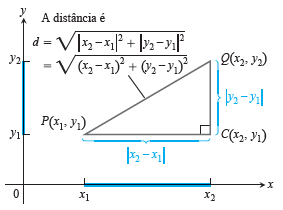
\includegraphics{graficodistancia.png}
    \caption{Descrição da imagem}
    \label{fig:exemplo}
\end{figure}